\documentclass{beamer}
\usepackage[utf8]{inputenc}
\usetheme{Madrid}
\usecolortheme{beaver}

% Setup figure insertion
\graphicspath{ {figures/} }

% Define title options
\title[Auditory Trilateration]{Auditory Localization using Trilateration in Two Dimensions}
\subtitle{Final Project in DT Signals \& Systems}
\date{2018}

\author[Seaborn, Lane]{A.~Seaborn\inst{1} \and T.~Lane\inst{2}}

\institute[BU]
{
  \inst{1}
  Department of Electrical \& Computer Engineering\\
  Bradley University
}

\date[FA18]{ECE 301, FA18}

% Customize TOC coloring
\setbeamercolor{section in toc}{fg = red}
\setbeamercolor{section number projected}{bg = red, fg = black}
\setbeamercolor{subsection in toc}{fg = red}
\setbeamercolor{subsection number projected}{bg = red, fg = black}


\begin{document}



%
%-----------------------------------------------------------------------------------------------------------|| TITLE
%

\frame{\titlepage}


%
%-----------------------------------------------------------------------------------------------------------|| TABLE OF CONTENTS
%

\begin{frame}

	\frametitle{Table of Contents}
	
	\tableofcontents
	
\end{frame}


%
%-----------------------------------------------------------------------------------------------------------|| PROBLEM STATEMENT
%

\section{Problem Statement}
\begin{frame}

	\frametitle{Problem Statement}
	
	"\textit{Use computer microphones from at least 3 laptops to record a 'gun shot' sound from a speaker.}``

	\begin{itemize}
		\item Develop an algorithm to determine the location of “gun shot”
		\item Vary the volume of gun shot, the distance of “gun shot” to study the robustness of your algorithm
		\item Add different background noise to the “gun shot” data, then analyze your performance of algorithm
	\end{itemize}
	
\end{frame}


%
%-----------------------------------------------------------------------------------------------------------|| PROBLEM APPROACH
%

\section{Problem Approach}
\begin{frame}

	\frametitle{Problem Approach}
	
	Use a microcontroller to sample three microphone sensors and use trilateration to find the source of the sound (in this case a buzzer triggered by an interrupt).
	
	\vspace{0.5cm}
	
	Two approaches:
	\begin{itemize}
		\setlength{\itemindent}{4.5em}
		\item[\textbf{Amplitude - }] find a predictable relationship between distance and amplitude, then run the trilateration.
		\item[\textbf{Time Diff - }] detect the differences between arrival times and multiply by the speed of sound to find the distance.\footnote{$343 \: m / 1000 \: ms$}
	\end{itemize}
	
	\begin{definition}
		Trilateration is a localization method which uses known points and their distances to an unknown point to find it. 
	\end{definition}

\end{frame}


%
%-----------------------------------------------------------------------------------------------------------|| DATA COLLECTION
%

\section{Data Collection}
\subsection{Experiment Setup}
\begin{frame}

	\frametitle{Data Collection - Experiment Setup}
	
	\begin{figure}[h!]
		\centering
		\includegraphics[width = 0.85\textwidth]{Layout.JPG}
		\caption{Sensor arrangement.}
	\end{figure}

\end{frame}


\begin{frame}

	\frametitle{Data Collection - Experiment Setup}
	
	\begin{figure}[h!]
		\centering
		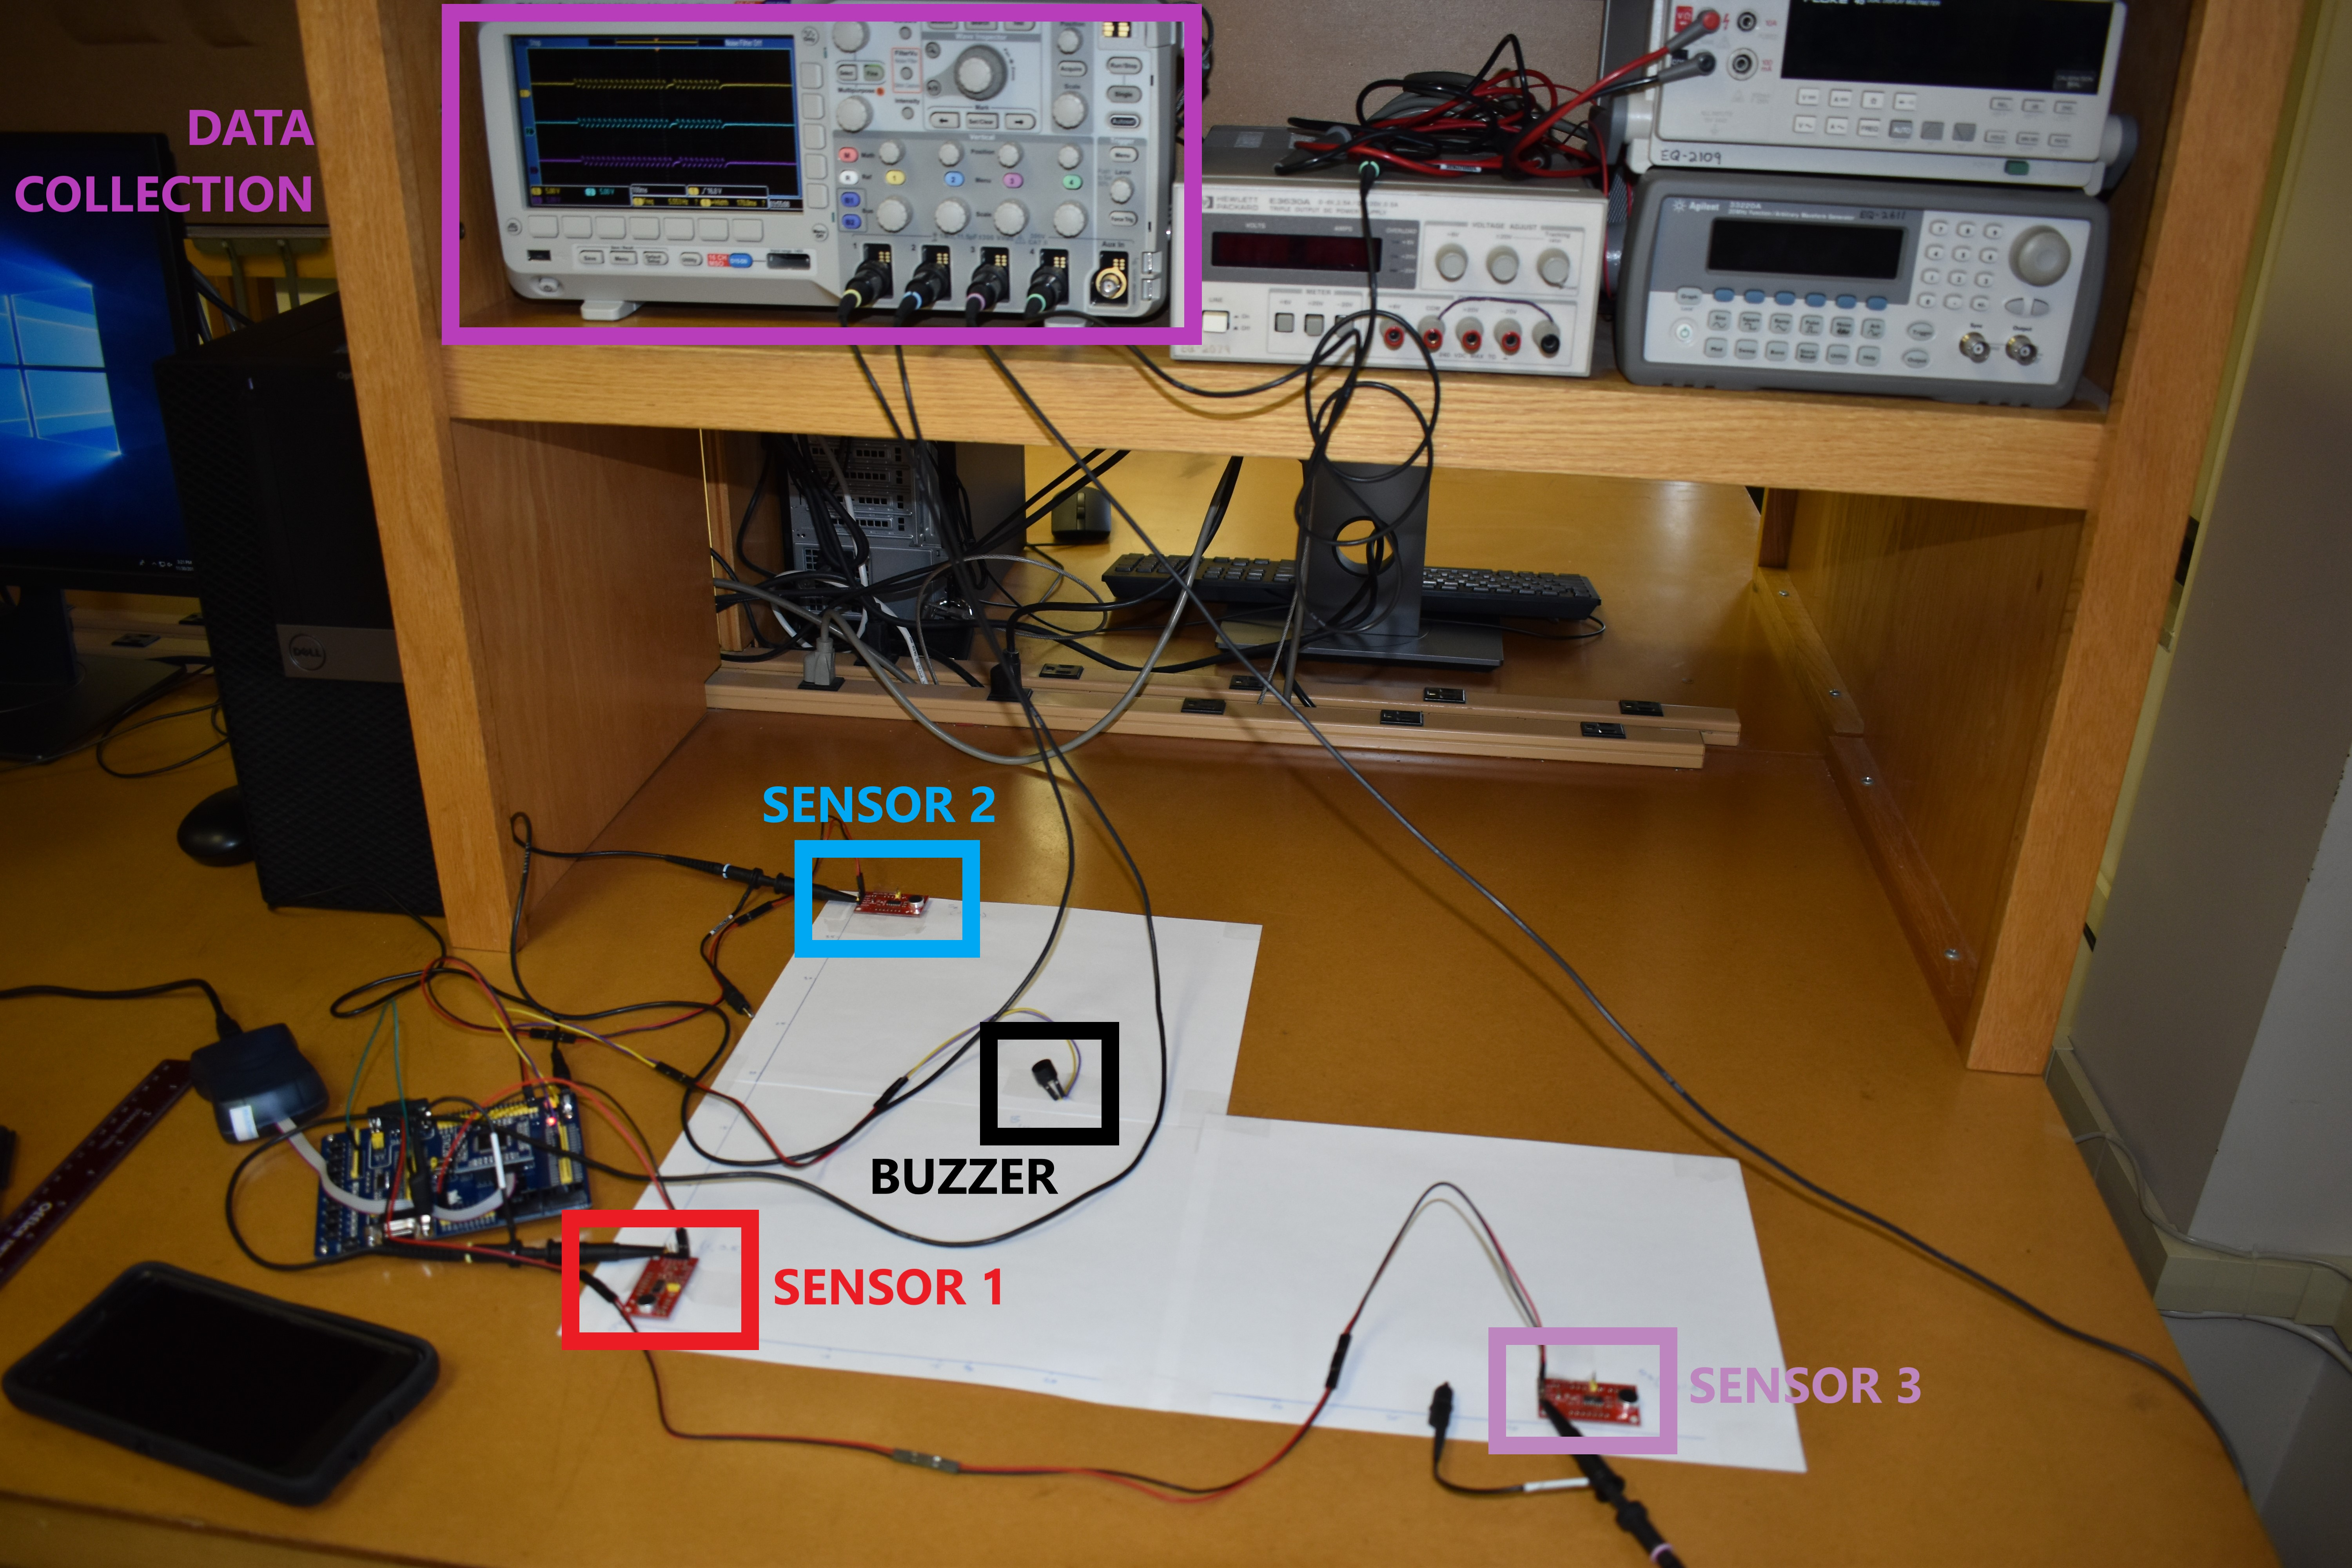
\includegraphics[width = 0.85\textwidth]{Layout-Captioned.JPG}
		\caption{Sensor arrangement explained.}
	\end{figure}

\end{frame}


\begin{frame}

	\frametitle{Data Collection - Experiment Setup}
	
	\begin{figure}[h!]
		\centering
		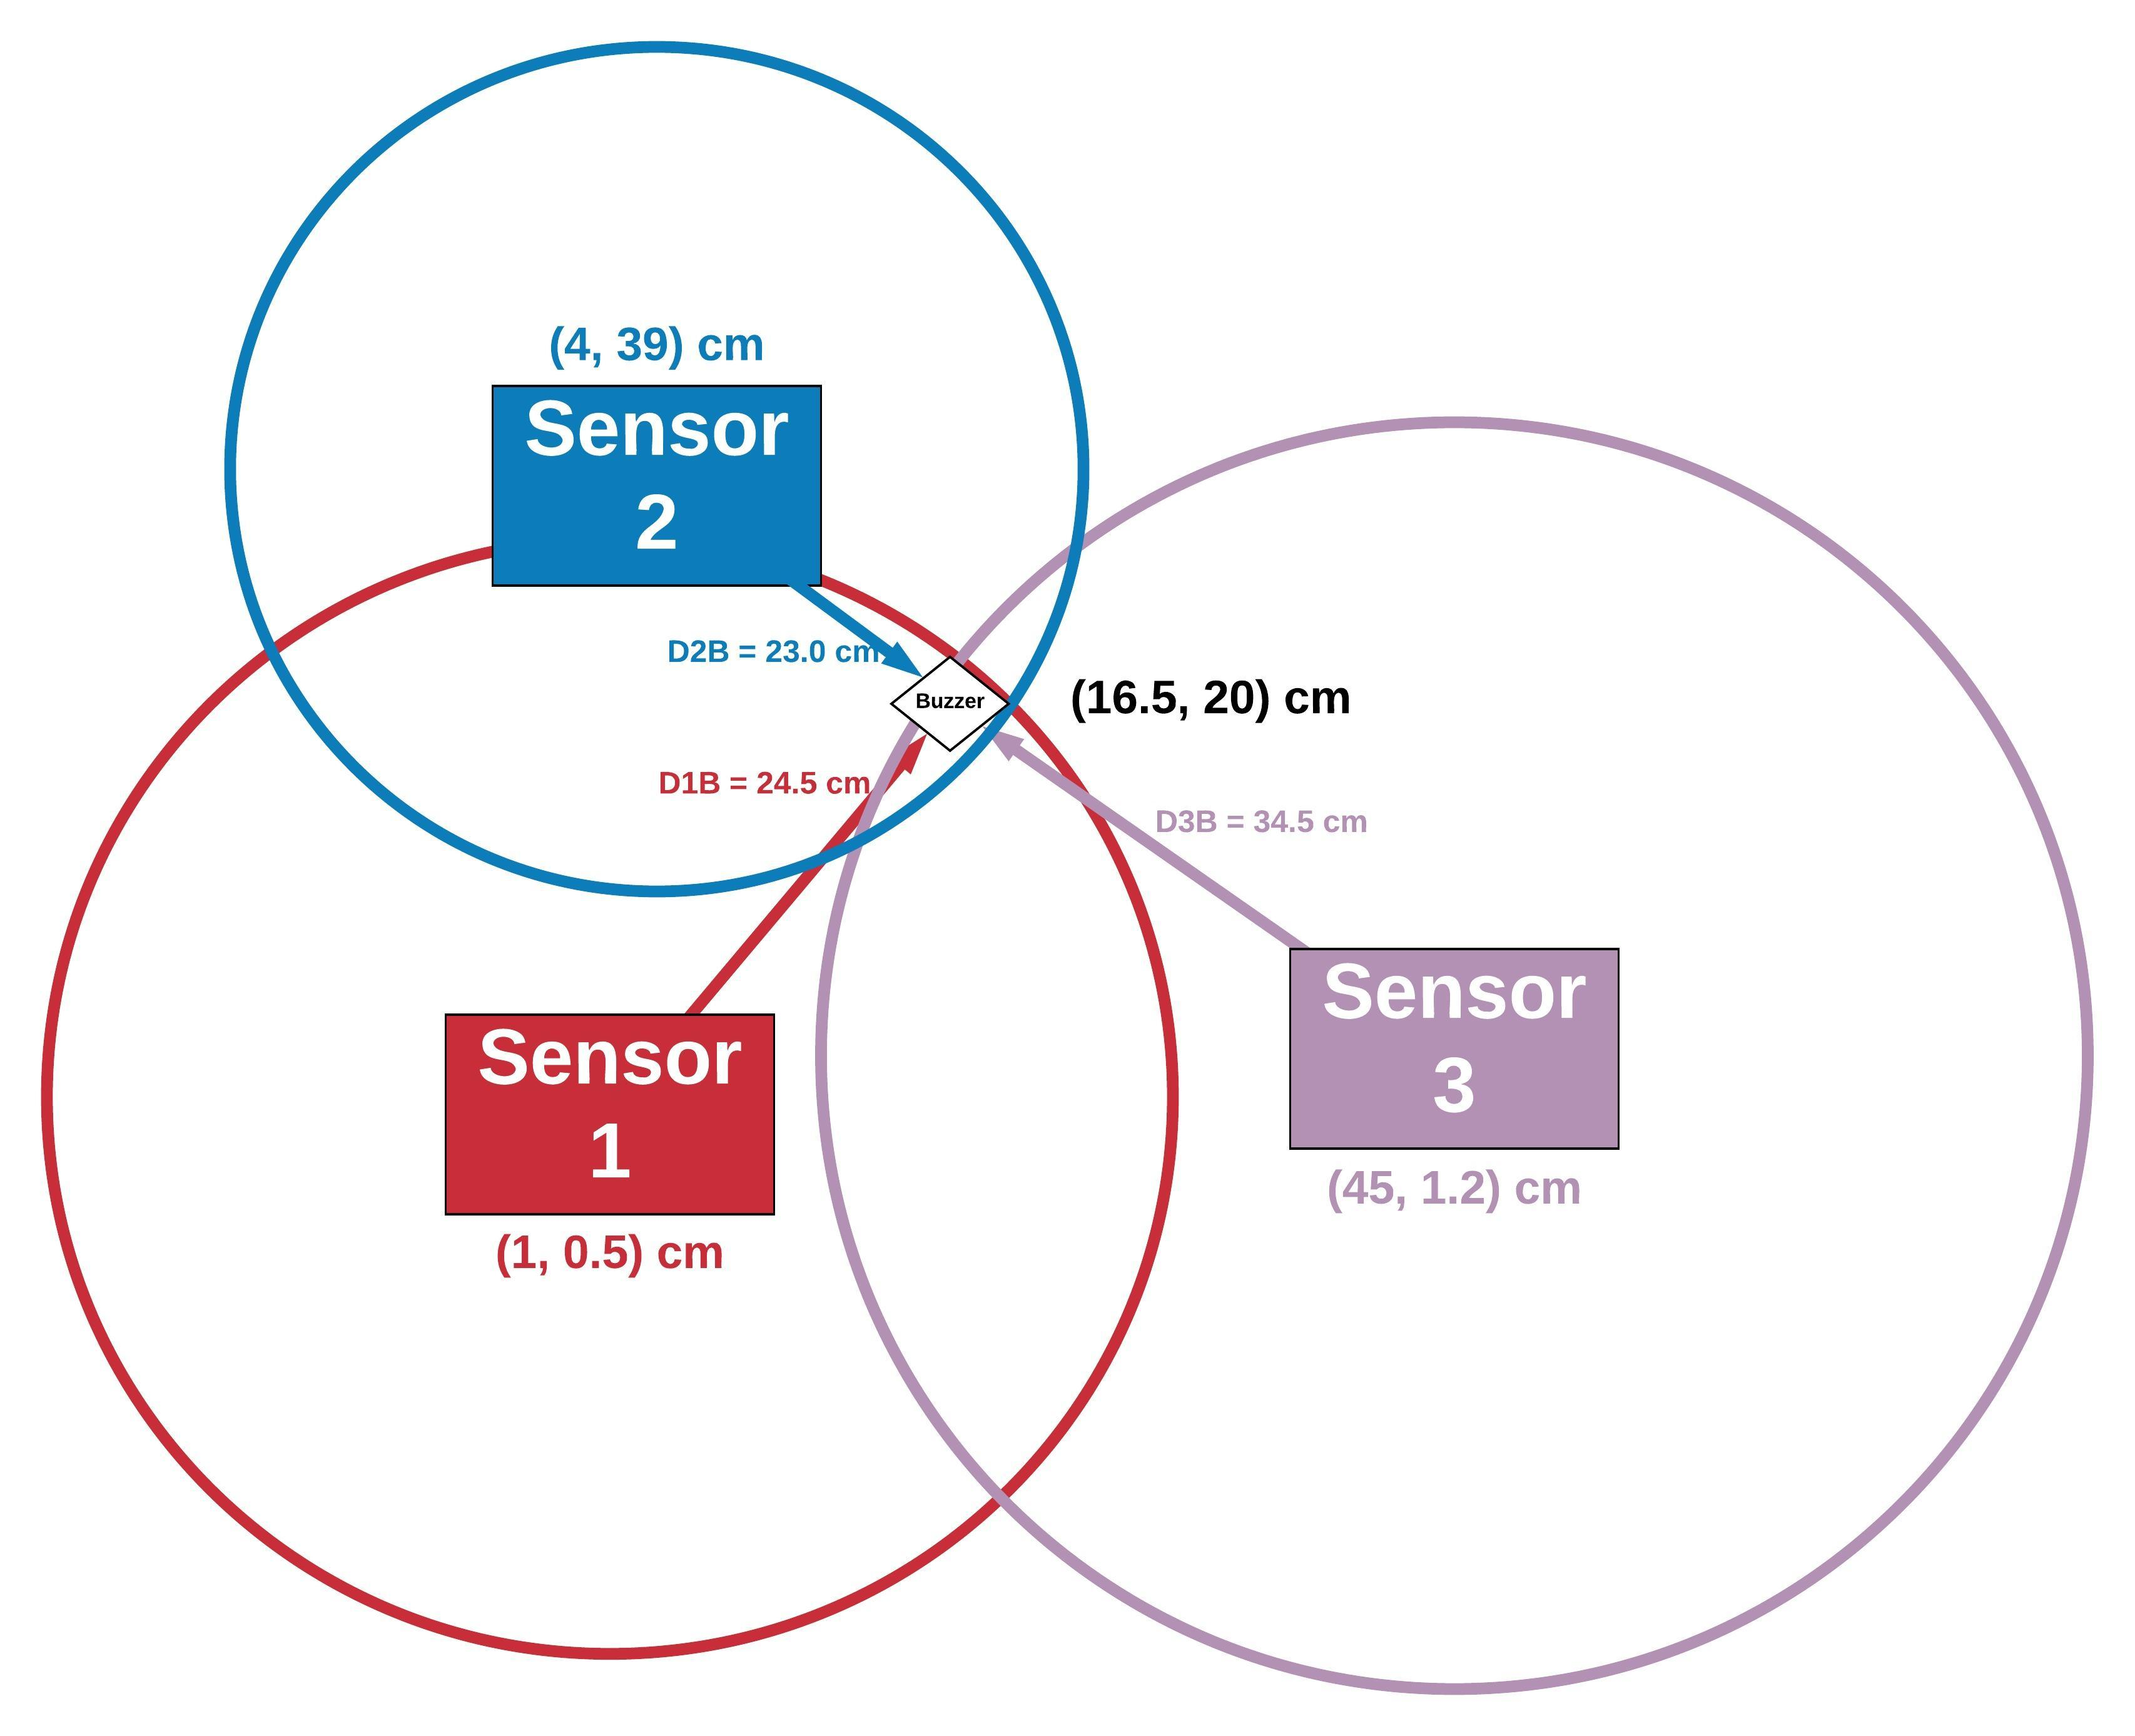
\includegraphics[width = 0.65\textwidth]{Experiment-Setup-Large.jpeg}
		\caption{Experiment diagram.}
	\end{figure}

\end{frame}


\subsection{Experiment Results}
\begin{frame}

	\frametitle{Data Collection - Experiment Results}
	
	% Include data sample figure
	\begin{figure}[h!]
		\centering
		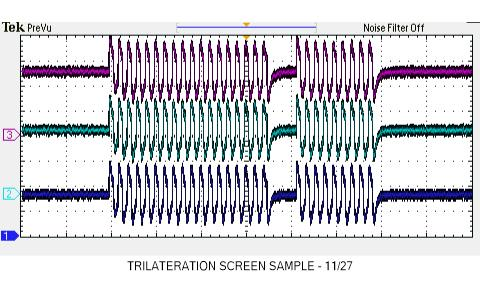
\includegraphics[width = 0.65\textwidth]{DataSample.jpg}
		\caption{Data collection results\footnote{See this youtube video for a demonstration
\url{https://youtu.be/WUPCAduKl10}}.}
	\end{figure}

\end{frame}


\begin{frame}

	\frametitle{Data Collection - Experiment Results}
	
	% Put text and a figure side by side
	\begin{tabular}{cl}  
		\begin{tabular}{c}
		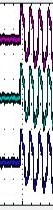
\includegraphics[height=5cm, width=3.5cm]{DataSampleDelay.jpg}
		\end{tabular}
		& \begin{tabular}{l}
		\parbox{0.5\linewidth}{%  change the parbox width as appropiate
		Believe it or not, there is a delay in the arrival times of the audio samples, allowing us to apply the time difference approach.   
    		}
         \end{tabular}  \\
	\end{tabular}

\end{frame}


%
%-----------------------------------------------------------------------------------------------------------|| DATA ANALYSIS
%

\section{Data Analysis}
\subsection{Data Preparation}
\begin{frame}

	\frametitle{Data Analysis - Data Preparation}
	
	\begin{figure}[h!]
		\centering
		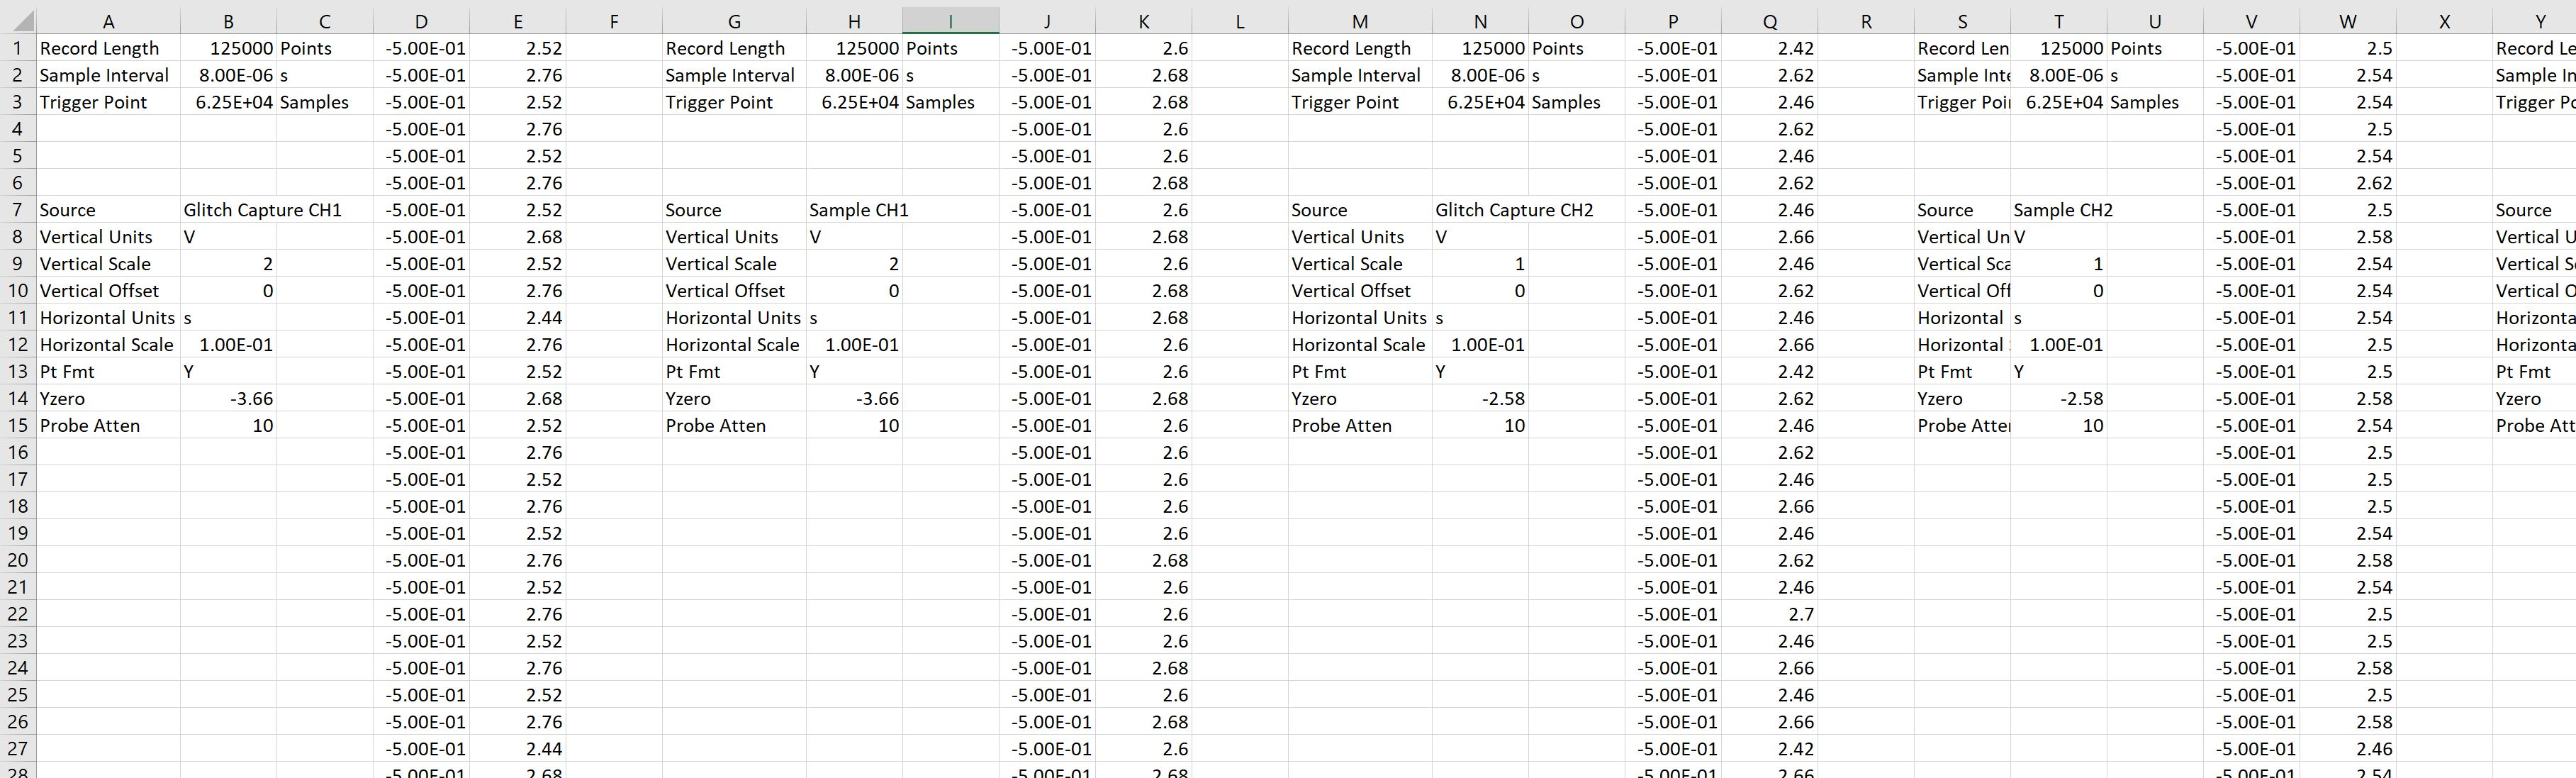
\includegraphics[width = \textwidth]{OscOutput.JPG}
		\caption{Oscilloscope data export format.}
	\end{figure}

\end{frame}


\begin{frame}

	\frametitle{Data Analysis - Data Preparation}
	
	\begin{figure}[h!]
		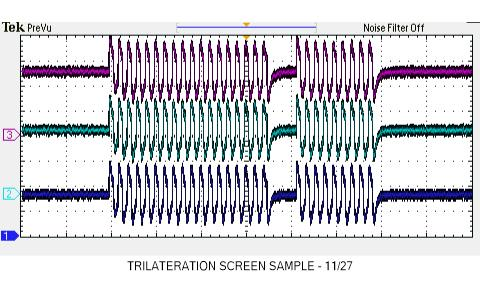
\includegraphics[width=0.45\textwidth]{DataSample.jpg}%		
		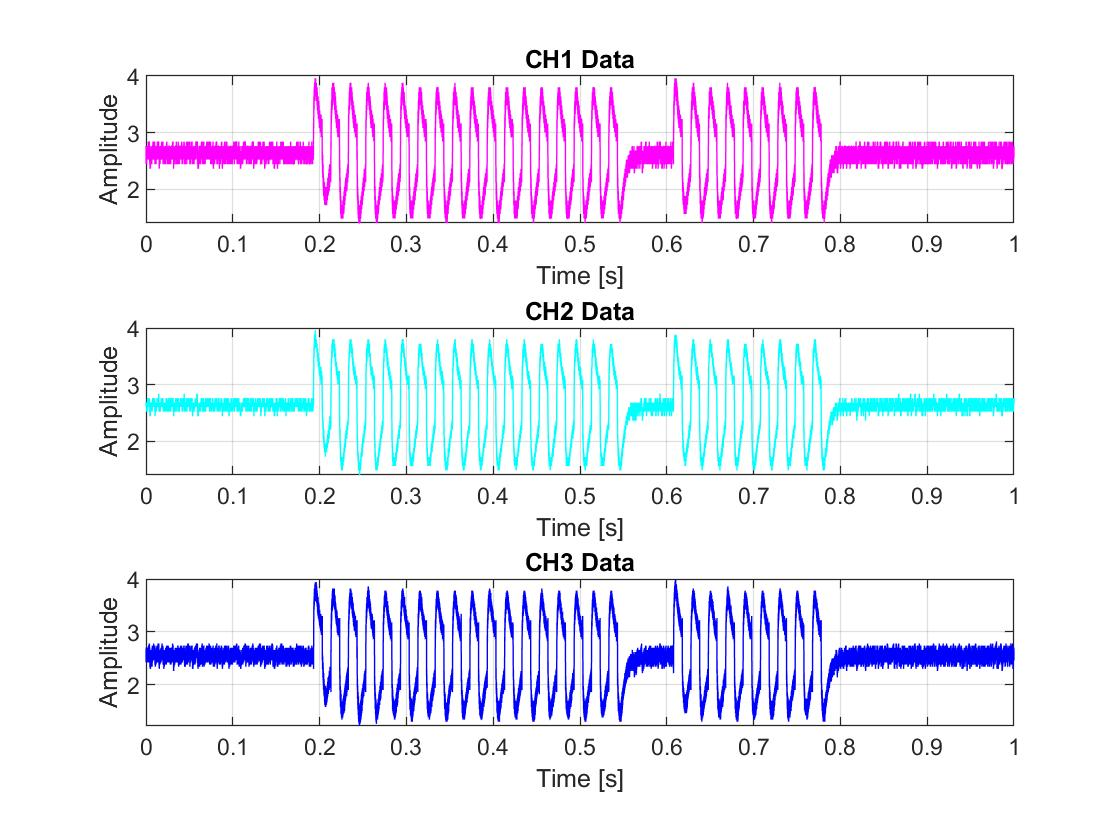
\includegraphics[width=0.45\textwidth]{MATLABdata.jpg}
		
		\caption{Comparison of data import.}
	\end{figure}
	
\end{frame}


\subsection{MATLAB Synthesis}
\begin{frame}

	\frametitle{Data Analysis - MATLAB Synthesis}
	
	% Put text and a figure side by side
	\begin{tabular}{cl}  
		\begin{tabular}{c}
		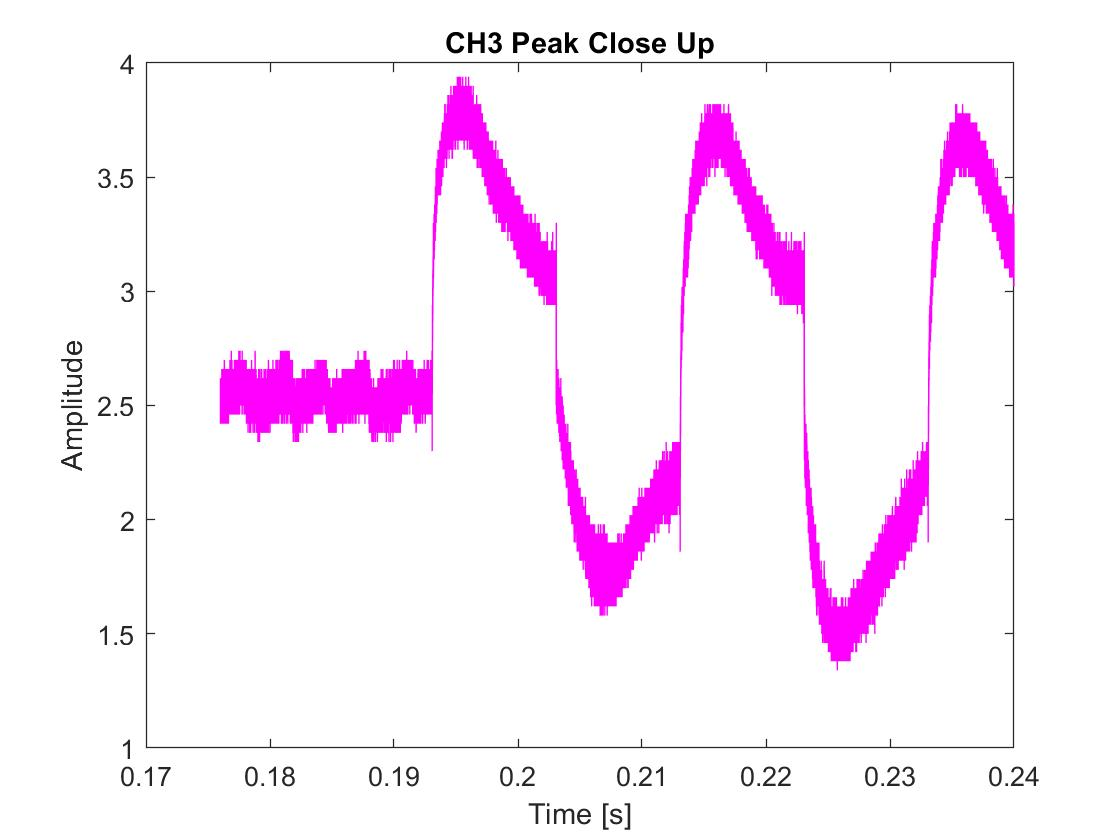
\includegraphics[width = 0.4\textwidth]{PeaksCloseup.jpg}
		\end{tabular}
		& \begin{tabular}{l}
		\parbox{0.5\linewidth}{%  change the parbox width as appropiate
		We can use findpeaks() to locate extrema in the data.
    		}
         \end{tabular}  \\
	\end{tabular}
	
\end{frame}


\subsection{Results}
\begin{frame}

	\frametitle{Data Analysis - Results}
	
	\begin{figure}[h!]
		\centering
		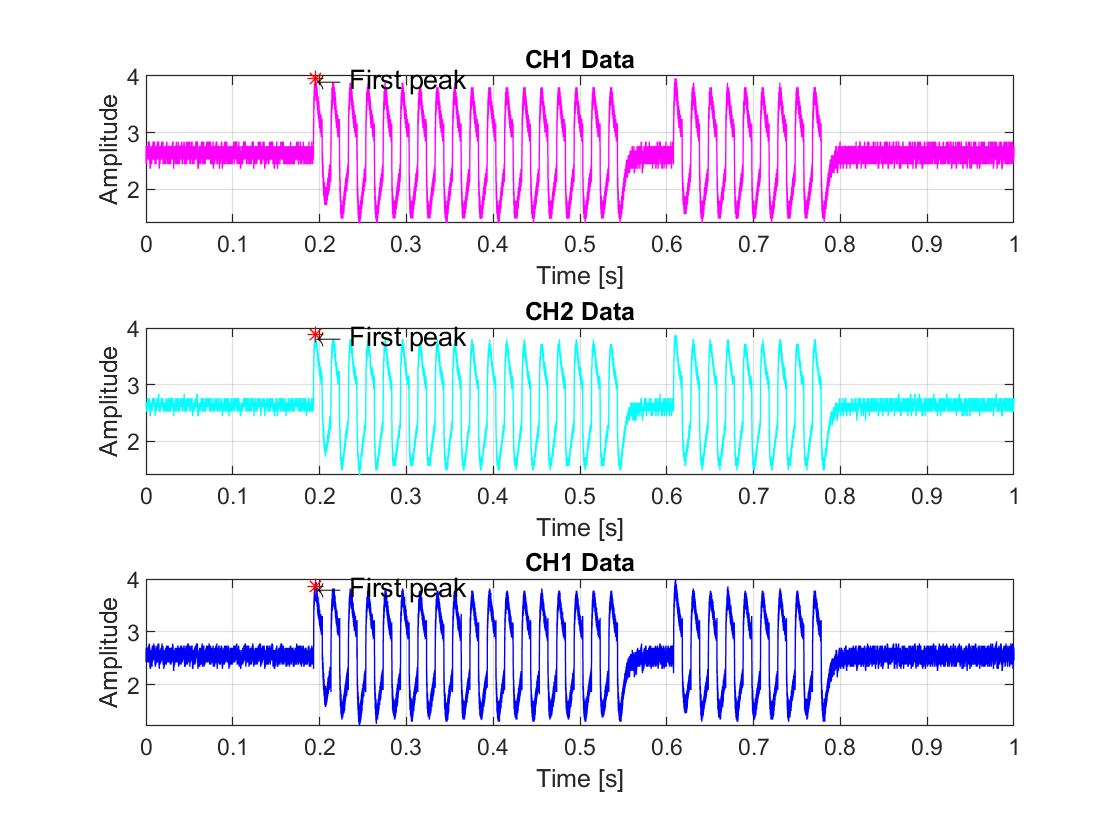
\includegraphics[width = 0.75\textwidth]{PeaksFound.JPG}
		\caption{MATLAB peak search results.}
	\end{figure}
	
\end{frame}


\begin{frame}

	\frametitle{Data Analysis - Results}
	
	\begin{figure}[h!]
		\centering
		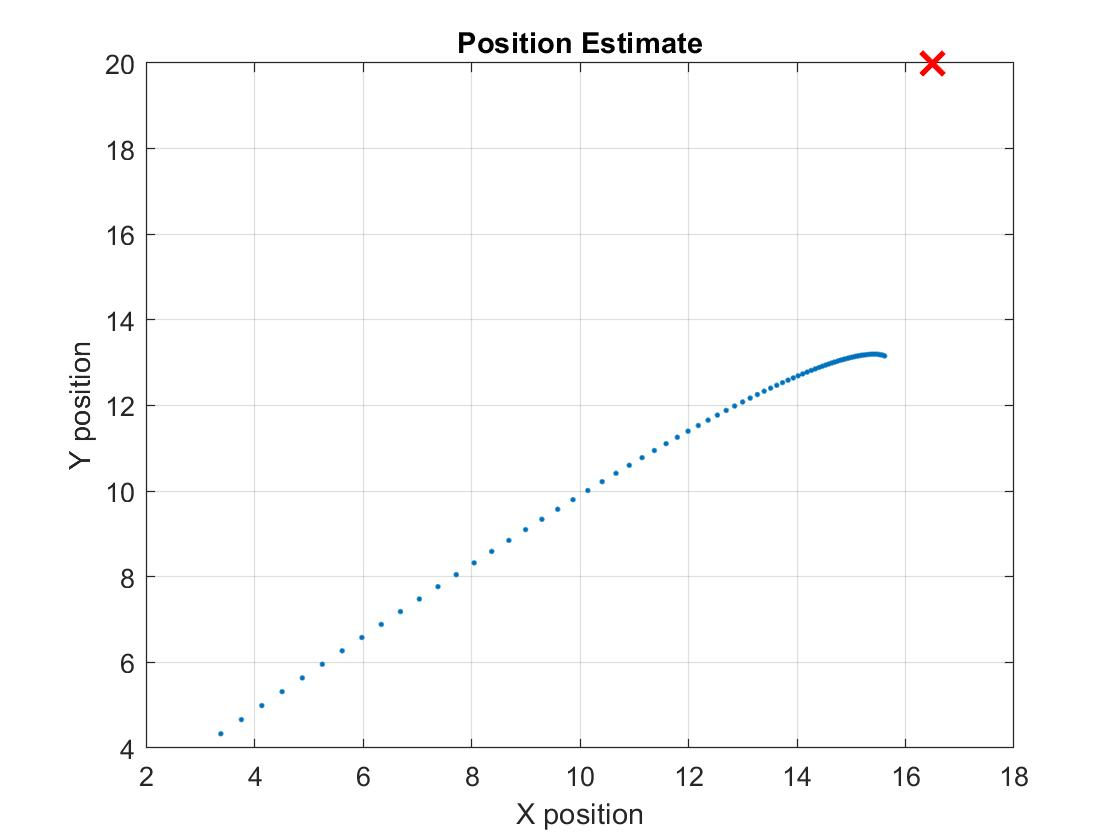
\includegraphics[width = 0.75\textwidth]{OptimizationResults.JPG}
		\caption{Trilateration results.}
	\end{figure}
	
\end{frame}


%
%-----------------------------------------------------------------------------------------------------------|| GOING FURTHER
%

\section{Going Further}
\begin{frame}

	\frametitle{Going Further}
	
	There are several areas for further development:

	\begin{itemize}
		\item<1-> Use the envelope to utilize the amplitude approach.
		\item<2-> Implement it in real time in the microcontroller.
		\item<3-> ...
	\end{itemize}

\end{frame}


%
%-----------------------------------------------------------------------------------------------------------|| QUESTIONS PAGE
%

\section{Questions}
\begin{frame}

	\frametitle{Questions}
	
	\begin{center}
	\begin{LARGE}
		\textbf{Questions?}
	\end{LARGE}
	\end{center}

\end{frame}



\end{document}

